% !TEX root = ../main.tex
\section{Background}

\subsection{Reinforcement Learning}

\paragraph{Problem formulation}

\paragraph{Common solutions}

\subsubsection{Reinforcement learning algorithm}
MarineGym comes with an implementation of Proximal Policy Optimization (PPO) out of the box \cite{chu2025marinegym}. The implementation is identical to the PPO in OmniDrones on which MarineGym was buildt \cite{xu2024omnidrones}.


\subsection{Recurrent policies}
% TODO: why memory (POMDP), LSTM/GRU equations. Moved from Related Work:
\begin{itemize}
  \item Problem: a forward-looking camera/sonar only observes the present;
        obstacles leave the field of view, so navigation is partially
        observable and needs a representation of space beyond the current
        frame.
  \item GRU \parencite{cho2014learning}: fewer gates, comparable to LSTM
        \parencite{chung2014empirical}.
\end{itemize}

\subsection{Convolutional neural networks}
% Moved from Related Work (End-to-end encoders)
Convolutional Neural Networks were first introduced in\textcite{lecun1998gradient}, and are widely adopted in the field of computer vision for their specific ability to encode variability in 2D shapes.

\subsection{Autoencoders and VAEs}
% Moved from Related Work (Encoders trained on reconstruction)
Another common way to compress data is with so called Auto Encoders (AE), which produce a compressed latent representation of the original input data \textcite{hinton2006reducing}. AEs work by defining two neural networks, one called an encoder and a decoder. The Encoder is constructed in a way so that the input dimensions are of the input data, while the output dimension is set to the desired compression dimension. The compressed representation is called a latent representation, and commonly denoted $z$. The decoder is on the other hand designed oppositely, so that the input dimension is matching the latent and the output dimension map back into the original input data. This is commonly visualized as a bottleneck as in figure \ref{fig:vae}. The Encoder and Decoder is jointly trained on a dataset passed through both networks sequentially, and are penalized with a loss that penalizes the difference between the input data and the reconstructed data. The latent representation, the encoder maps to will then retain most of the information in the original data while the dimensions are reduced. For images, convolutional encoders and decoders preserve spatial structure and shares their weights across images improving spatial understanding \cite{masci2011stacked}. Variational Auto Encoders (VAEs) are a common extention of AE, and are designed to keep latent representations resembling a normal distribution \cite{kingma2014auto}.

\begin{figure}[H]
    \centering
    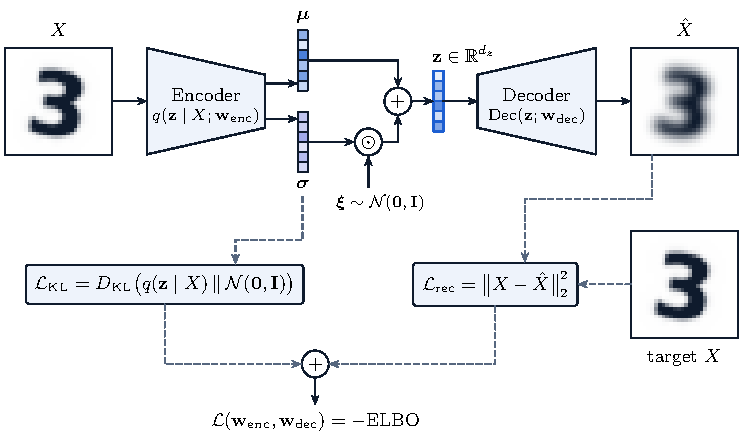
\includegraphics[width=1.0\linewidth]{figures/vae.pdf}
    \caption{Canonical Variational Auto Encoder (VAE)}
    \label{fig:placeholder}
\end{figure}

\subsection{Collision images}
% Moved from Related Work (Task-driven compression)
These images are generated by first detecting edges along the original image of which some of the edges are selected randomly to be used for meshes. The meshes in combination with a pinhole camera model used to render virtual meshes for the edge pixels of the image and internal image pixels are simply offset by the robot size. The images are ultimaly combined into an new image which represents the collision free distance projected along the central axis of the camera, representing the traversable distance by a robot of a specific size along the rays corresponding to each pixel in the image \cite{kulkarni2023task}. COME BACK TO THIS, its not right.

\subsection{Depth foundation model (DeFM)}
% TODO: skeleton. Input preprocessing, architecture, embedding used by the policy

\subsection{Underwater vehicle model}
\paragraph{Types of UUVs}

\paragraph{Sensor suit} typical sensor suit

\paragraph{Vehicle dynamics} The system dynamics in MarineGym are handled by decomposing the dynamics into a rigid-body term handled by PhysX, the physics engine budled with IsaacSim and a hydrodynamic term determined by Fossen's equation of motion \cite{amundsen2024aquaculture}. Where $\boldsymbol{\tau} \in \mathbb{R}^6$ is the vector of control forces and moments produced by the thrusters, $\boldsymbol{\nu} = [u, v, w, p, q, r]^\top$ is the vector of linear and angular velocities expressed in the body-fixed frame, and $\boldsymbol{\eta} = [x, y, z, \phi, \theta, \psi]^\top$ is the position and orientation (Euler angles) of the vehicle in the North-East-Down (NED) frame. The matrix $\mathbf{M}_{RB}$ is the rigid-body mass and inertia matrix, $\mathbf{C}_{RB}(\boldsymbol{\nu})$ contains the rigid-body Coriolis and centripetal terms, and $\mathbf{g}_{RB}(\boldsymbol{\eta})$ represents the gravitational force acting on the vehicle. The hydrodynamic contributions consist of the added mass matrix $\mathbf{M}_{A}$, which accounts for the inertia of the surrounding fluid accelerated with the vehicle, the corresponding added-mass Coriolis and centripetal matrix $\mathbf{C}_{A}(\boldsymbol{\nu})$, the hydrodynamic damping matrix $\mathbf{D}(\boldsymbol{\nu})$, which includes both linear and quadratic drag, and $\mathbf{g}_{A}(\boldsymbol{\eta})$, which represents the buoyancy force. Together, $\mathbf{g}_{RB}(\boldsymbol{\eta})$ and $\mathbf{g}_{A}(\boldsymbol{\eta})$ form the restoring forces and moments acting on the vehicle. The torque from the hydrodynamic forces is applied to the centroid of each submerged link every time the model is forward stepped. This does not include forces and torques introduced by the actuators.

\begin{beqn}
\boldsymbol{\tau} = \underbrace{\mathbf{M}_{RB}\dot{\boldsymbol{\nu}} + \mathbf{C}_{RB}(\boldsymbol{\nu})\boldsymbol{\nu} + \mathbf{g}_{RB}(\boldsymbol{\eta})}_{\text{Rigid-body term}} + \underbrace{\mathbf{M}_{A}\dot{\boldsymbol{\nu}} + \mathbf{C}_{A}(\boldsymbol{\nu})\boldsymbol{\nu} + \mathbf{D}(\boldsymbol{\nu})\boldsymbol{\nu} + \mathbf{g}_{A}(\boldsymbol{\eta})}_{\text{Hydrodynamic term}}
\label{eq:dynamics}
\end{beqn}

\paragraph{BlueRov2 Heavy in MarineGym}
In MarineGym the actuator model is split into a rotor dynamics model simulating the time dependent response of the rotor system, and a thrust generation model simulating which maps actuator states to the forces and torques. The thrust generation model for propellers is represented as a quadratic function with a dead zone. In this zone the thrust is set to be proportional to the deviation of rotational speed within predefined thresholds to account for nonlinear efficency variations? Each actuator generates their own force based on the input command and the actuator model, before they are individually applied to the corresponding actuator frame. All actuator configurations are fully configurable in MarineGym, however a built-in configuration of the T200 thruster from Blue  Robotics which is used in the BlueROV2 Heavy.

\subsection{Simulation}
\label{sec:marinegym}

\paragraph{MarineGym} MarineGym \cite{chu2025marinegym} is a GPU-accelerated framework for training control policies with RL for underwater robotics. MarineGym provides GPU native hydrodynamics, accounts for environmental disturbances, a toolkit for Domain Randomization (DR) and supports multiple UUV- and actutor models. Allowing for large-scale paralellizartion of simulations, outperforming alternative simualtors such as HoloOcean, DAVE ans Stonefish which relies on CPU-based multiprocessing. MarineGym~\cite{chu2025marinegym}  is built on NVIDIA Isaac Sim, a robotics simulator that combines the PhysX physics engine, RTX rendering and sensor simulation. In GPU mode, PhysX runs as CUDA kernels, so the rigid-body calculations are spread across the GPU's many cores. MarineGym accesses the simulation through Isaac Sim's tensor application programming interface (API), which lets PhysX and PyTorch share the same GPU memory. Because Isaac Sim has no native support for hydrodynamic forces, MarineGym adds a custom plugin, written as PyTorch tensor operations, that computes the hydrodynamic terms of Fossen's equations of motion and applies them to each vehicle at every simulation step. Physics, hydrodynamics and policy inference therefore all run on the GPU, and simulation data never has to be copied to the CPU between steps.

\paragraph{Other candidate simulators} Stonefish etc.

\paragraph{Sensor emulation} Sonar-and camera emulation (RGB, Depth and Segmentation) are not explicitly added features added by MarineGym. However, camera emulation is available in Isaac Sim and is a trivial extension to MarineGym. Sonar emulation is also not supported by MarineGym, and is usually implemented manually as raycast.
